\question
\begin{lstlisting}
public class Horse {                          
    Horse same;                             
    String jimmy;                
    public Horse(String lee) {
        jimmy = lee;
    }
    public Horse same(Horse horse) {
        if (same != null) {
            Horse same = horse;
            same.same = horse;
            same = horse.same;
        }
        return same.same;
    }
    public static void main(String[] args) {
        Horse horse = new Horse("you've been");
        Horse cult = new Horse("horsed");
        cult.same = cult;
        cult = cult.same(horse);
        System.out.println(cult.jimmy);
        System.out.println(horse.jimmy);
    }
}
\end{lstlisting}

\begin{parts}
\part What would Java display?
\begin{solution}[0.5in]
\begin{verbatim}
horsed
you've been
\end{verbatim}
\end{solution}

\part Draw the box-and-pointer diagram after the \texttt{main} method has executed.
\begin{solution}[2in]
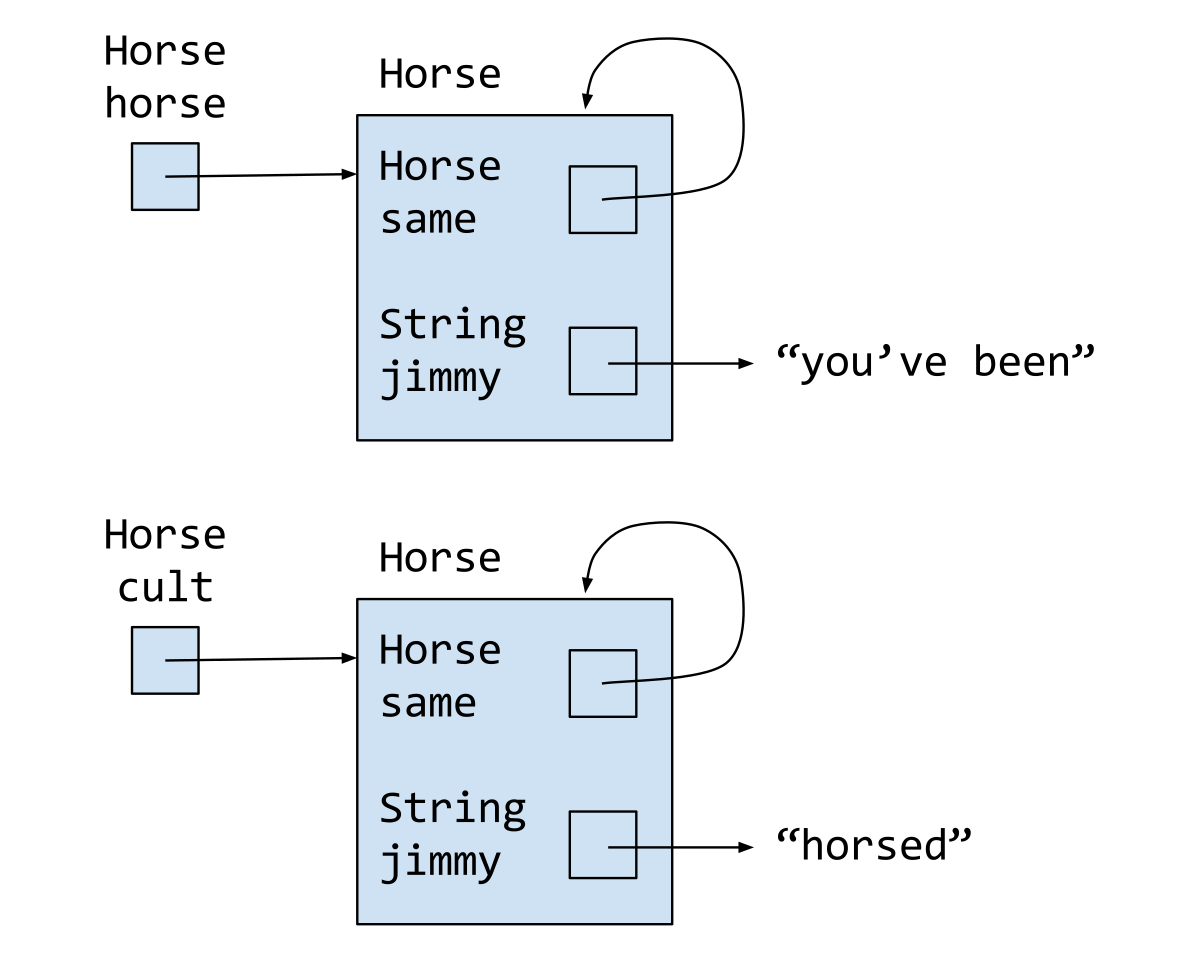
\includegraphics[width=0.5\textwidth]{samehorse}
\end{solution}
\end{parts}